
% Supõe-se que, na introdução, tenha sido posto a definição do problema de SQA como a necessidade de garantir um sinal de boa qualidade, seja para humanos não cometerem enganos, seja para modelos preditivos serem capazes de estimar com acurácia.

\glsreset{SQA}

This chapter is dedicated to exploring similar case studies and works in the area of \gls{SQA}, especially for cardiological signals. \gls{SQA} involves a wide range of problems in signal processing technologies, and it is not exclusive to the medical domain. Actually, its origins relate to the old communication systems, when researchers published their first works on the information theory 	in the 1920s and 1930s. One example of such foundational \change{publications is the work of Rice \cite{origins-1},} in which he analyzes the statistical properties of communication device noises. Another example is \change{the work of Shannon \cite{origins-2}}, which introduces fundamental concepts in communication systems. In that millennium, studies already used the concept of \gls{SQA} \change{\cite{origins-3, origins-4}}. We can see samples of this in the 1980s, such as \change{the work of Stehle \cite{origins-3},} which proposed an algorithm for assessing the quality of shortwave broadcast signals, trying to objectively measure the human perception of the signal message intelligibility. Some of its conclusions are useful in the \gls{SQA} in clinical contexts, such as the high degree of subjectivity in the human idea of quality. This makes labeling datasets properly fundamental to reflect this concept of quality in the proper evaluation of the developed \gls{SQA} algorithms.
	
Past the 20th century, the \gls{SQA} of physiological signals begin to become popular. Particularly, the early 2000s had several works in the subject. One of them is the work of Wang et al. \cite{2000s-1}, which proposed a \gls{ECG} \gls{SQA} method based on the difference between the areas of distinct QRS complexes. The work proposed comparing the cumulative histograms of different \gls{ECG} leads to assess its qualities. Later,  Li et al. \cite{2000s-2} suggested the combination of multiple quality indices and \gls{HR} to assess \gls{ECG}. Another work, by Deshmane et al. \cite{2000s-3}, posed the thresholding based on the Hjorth parameters~\cite{hjorth-parameters} to assess the quality of \gls{PPG} signals. Afterwards, Zhang et al. \cite{2000s-4} elaborated an \gls{ABP} signal quality assessment metric based on the \gls{EDSS} and \gls{SESS} features. Through those works, the researchers proposed quantifying the \gls{SQA} in a metric \cite{2000s-2, 2000s-3, 2000s-4}. A name that they used to refer to this metric was \gls{SQI} \cite{2000s-2, 2000s-3}.


\section{Quality assessment of physiological signals}

Among the variety of physiological signals, the \gls{ECG} is prevalent in the literature. This signal has multiple applications, such as disease classification, heartbeat type detection, biometric detection and emotion recognition \cite{ecg-1}. There are plenty of works in the \gls{SQA} of ECG signals. In one of them, Naseri et al. \cite{ecg-2} proposed two features for the estimation of a classification \gls{SQI} of multi-channeled \gls{ECG}s. One feature consists of verifying if two energy-like indices, measured in decibels, are within an admissible range. The other feature result from randomly choosing a target lead, feeding a \gls{FFNN} with array of derivatives of all leads to reconstruct the targeted lead and finally comparing the original target lead to its artificial version with correlation analysis. Therefore, the \gls{ECG} is present in the \gls{SQA} literature.

\change{Also, there are other publications on the \gls{ECG} \gls{SQA}}. For instance, in 2017, Orphanidou et al. \cite{ecg-3} introduced a feature based on the extraction of the \gls{HRV} of \gls{ECG} signals. The method decomposes this new signal into wavelets with different frequency ranges and calculates the entropy of each of them, forming a feature vector. This vector feeds a \gls{SVM}, which classifies the signal as acceptable or not. Later, Shahriari et al. \cite{ecg-4} developed an image-based feature that measures the Structural Similarity Measure between the input plot image, containing each signal channel Cartesian graph, and multiple template plot images of similar shape selected from the training dataset by using clustering analysis. One year later, Moeyersons et al. \cite{ecg-5} proposed transforming the signal using the Auto Correlation Function and extracting simple features from it. In 2024, Huerta et al. \cite{ecg-6} generated phase space plots, such as Poincaré plots, and discretized them into a grid where each cell is the logarithm of the number of points contained in that cell. Thus, the \gls{SQA} literature for \gls{ECG} \change{ranges multiple works}.

\change{Besides the relevance of the \gls{ECG}, the \gls{PPG} has increased in popularity as an alternative to it.} In fact, its number of related articles published from 2013 to 2023 has increased by 176\% \cite{ppg-1}. \change{However, as previously presented in Chapter \ref{Introducao}, the \gls{PPG} is also susceptible to noise, fact that led to the development of \gls{PPG} \gls{SQA} methods.} A sample of this literature is the work of Li et al. \cite{ppg-2}, which poses the measurement of a \gls{SQI} through the application of the \gls{DTW} technique to measure the signal disparity to an established template. These authors then fed this \gls{SQI} and some others to a \gls{MLP} and to a self-made rule function, predicting a unique \gls{SQI}. Experiments on private annotations on the MIMIC II dataset resulted on the \gls{MLP} achieving the highest accuracy, 95.2\%. Another sample is the work of Papini et al. \cite{ppg-3}, in which they proposed a method that first segments the input signal by finding all negative local minima points. Then, the method creates a template signal by calculating the Dynamic Time Warping Barycenter Average of the signal segments. Finally, it calculates the \gls{SQI} for each beat by comparing them to the template. This method obtained above 95\% sensitivity and positive predictive values on two public datasets. Therefore, it is possible to achieve good predictive quality in the \gls{SQA} of \glspl{PPG}.


According to Such~\cite{such2007motion}, \gls{SQA} methods in biomedical signals generally fall into two categories: single-parameter and multiparameter approaches. Unlike single-parameter methods, multiparameter techniques utilize additional sensors that provide information related to the motion or the \gls{PPG} itself. Examples of these additional sensors include accelerometers~\cite{nabavi2020robust, tuauctan2015characterization} and optical source-detector pairs with peak responses beyond the red-infrared wavelength spectrum~\cite{zhang2019motion}. Some studies generate reference noise signals internally from the impaired \gls{PPG} segments, reducing the need for extra hardware~\cite{ram2011novel, raghuram2016use}. Additional sensor channels can also transmit data about the same or a similar physiological indicator that reacts differently to artifacts. Nevertheless, the use of measured or synthetic reference signals to detect contaminated \gls{PPG} segments often involves adaptive filtering, which, aside from its high computational and mathematical complexity, may require significant amounts of data and time to reach an optimal solution.



In contrast to the techniques mentioned earlier, \gls{SQA} methods that do not rely on measured or synthetic reference signals (i.e. referenceless methods) may be better suited for wearable, real-time applications, since they eliminate the need for additional data collection and processing. In this context, \gls{ML} has made significant strides in this area by enabling the classification of \gls{PPG} signals into `reliable' or `unreliable' based on the extraction of distinguishing information and the recognition of complex patterns, either automatically or with minimal human involvement~\cite{janiesch2021machine}. 


%\subsection{PPG SQA}
		
One characteristic of the \gls{PPG} \gls{SQA} literature is the presence of both supervised and unsupervised machine learning approaches. Supervised learning involves learning features with the presence of labels. This allows the machine learning model to have access to more information in the learning process, \change{but at the cost of more training computational expense}. Multiple works in the \gls{SQA} literature are supervised. Per example, Mohagheghian et al. \cite{ppg-sqa-1} introduced a method to improve feature selection algorithms by ensembling feature subsets into a majority voting schema. A machine learning algorithm determines the voting threshold, such as AdaBoost, \gls{SVM}, \gls{KNN} and discriminant analysis. Among those predictors, the AdaBoost presented the best performance in terms of \gls{ROC AUC} and accuracy. Furthemore, the method achieved accuracies of 91,55\%, 92,29\% and 95,86\% on, respectively, the DeepBeat, UMMC Simband, and MIMICIII datasets. This result is competitive to other three compared methods, despite the labeled quality scores are not publicly available. As another example, Tiwari et al. \cite{ppg-sqa-2} proposed transforming the signal into a Modulation Spectrogram representation and, then, extracting features from it for subsequently feeding them to a machine learning model. Experiments compared the method to various \glspl{SQI} by feeding them to a logistic regressor. Tests involved three wavelengths: red, green and infrared. The results showed that the method outperformed the others \glspl{SQI} by 21.3\% \gls{BACC} for green, 21.6\% \gls{BACC} for red, and 19.0\% \gls{BACC} for infrared wavelengths. A final example is the work of Miranda et al. \cite{ppg-sqa-3}, in which the \gls{SQA} results from the application of a Interval Type-2 Fuzzy Logic system. Experiments on a private dataset lead to 77\% and 93.72\% \gls{MCC} and \gls{ACC}, respectively. However, one observation is that most of the experiments used originally unlabeled datasets, which make those results unreproducible. 
	
On the other hand, unsupervised learning dismisses labels in the learning process. Even though this approach gives less information to the trained model, this makes the model independent of specialists guidance and its biases. As opposed to most works in the \gls{SQA} literature, some works present unsupervised methods. For example, Singha et al. \cite{ppg-sqa-4} propose extracting entropy and statistical features from the input signal and feeding them to a Self-Organizing Map. Experiments on a private dataset resulted in 92.01\% accuracy in ternary classification. As another example, Mahmoudzadeh et al. \cite{ppg-sqa-5} proposed extracting features from the time and frequency domains and feeding them to a Elliptical Envelope Algorithm. This method achieved 97\% and 93\% F1-Score on ``Reliable'' label for, respectively, intra and inter subject testing on a private dataset. Additionally, the combination of the supervised and unsupervised methods can produce semi-supervised methods, such as the method of Feli et al. \cite{ppg-sqa-6}, which feeds features to a Semi-Supervised One Class \gls{SVM}, training it only on samples labeled as ``Reliable''. Comparing this semi-supervised approach to rule-based, unsupervised, supervised and deep learning methods lead to the proposed method surpassing all of them in terms of F1-Score for ``Reliable'' class with 99\% value on a private dataset. However, likewise the supervised works, most datasets and its testing labeling are not public.		

Another characteristic of the \gls{PPG} \gls{SQA} literature is the existence of the \gls{CA} identification problem. The \gls{CA} is the presence of an anomalous cardiac rate or rhythm without a physiological reason \cite{arrhythmia-1}. This medical condition is an obstacle in the design of \gls{SQI}, since, in contrast to arrhythmic individuals, normal cardiac signals are periodic. Some features assume that the signal is periodic. This assumption can result in signals with arrhythmia being rejected as unreliable signals, leaving patients \change{with the \gls{CA} condition} misdiagnosed. Pereira et al. \cite{arrhythmia-2} conducted experiments on a private dataset that contains cases of \gls{AF}, a type or arrhythmia. In this experiment, 40 features used in previous studies fed a \gls{SVM}, which achieved an average accuracy superior to 94\%. That accuracy was far higher than other existing methods, which the researchers also tested. Therefore, abundant feeding a machine learning algorithm with features and training it on datasets with arrhythmia cases already present an improvement in the detection of those special cases.

In sequence, two studies adopted a similar approach to the one mentioned in the past paragraph to attack the arrhythmia problem. In the first study, Pereira et al. \cite{arrhythmia-3} fed several features to three classifiers: \gls{SVM}, \gls{KNN} and Decision Tree. Similarly to their previous study, experiments on a private dataset demonstrated that the \gls{SVM} was the best of all classifiers and it obtained above 95\% surpassing the methods of other studies. The second study, by Pereira et al. \cite{arrhythmia-4}, also included the \gls{SVM} method, but added to the experiment deep learning models. The study contemplated both one-dimensional (1D) and bidimensional (2D) deep learning models, with the first receiving the raw signal and the second receiving its Cartesian plot image. Experiments on private data with presence of \gls{AF} showed that the ResNet18 model was the best, with 98.5\% accuracy. That last study highlighted that deep learning models have the potential to surpass conventional methods even with the presence of arrhythmic events. The next section further explores the use of deep learning in the literature.  

\section{Signal quality assessment using deep learning}
\label{sec:deep_learning}

Methods based on \gls{DL} have demonstrated the potential to achieve a higher accuracy when compared with feature-based models, even in the presence of \gls{CA}. On one hand, differently of hand-crafted features, \gls{DL} automatically extracts features from the input signal, creating models that are adaptable to different dataset training contexts. Additionally, a high quality dataset can provide resources for the \gls{DL} model to be robust to variations on the signal conditions. On the other hand, not only it creates a black-box that does not explain the reasons why the model attributed a certain \gls{SQI}, but also requires large amounts of data to properly adjust the model parameters. Despite this, \gls{DL} is worth exploring since it can provide the accuracy and robustness that the medical applications require. 

In this context, several studies proposed the application \glspl{CNN} \change{receiving the one-dimensional input signal}. For instance, Naeini et al. \cite{deep-learning-1} designed a 1D \gls{CNN} to extract a binary \gls{SQI}. Tests on a private dataset with data of three devices lead to 85\% F1-score for the ``Reliable'' class. Alike, Zanelli et al. \cite{deep-learning-2} employed a self-made 1D \gls{CNN}, but examined the effect of transfer learning as well. They conducted the experiment on three private datasets. It starts training the model mostly on one dataset, in which it achieved an accuracy of 99.8\%. Then, for each remaining database, they fine-tuned the the model with little training and tested on it. This procedure resulted on the 93\% and 81\% accuracies on the second and third datasets, respectively. Additionally, the model trained solely on the second database scored lower, 86\%. Those results indicate that not only \change{1D \glspl{CNN} can achieve high accuracy in \gls{SQA}} but also \change{it is possible to} transfer its learned features over different databases to improve its performance.

In a different light, some works go beyond the simple application of such \glspl{CNN}. The research of Lucafo et al. \cite{deep-learning-3}, per example, introduced a hybrid-model for quality assessment, which combines a 1D \gls{CNN} with a rule-based approach. This rule can bypass the utilization of the \gls{CNN} by verifying if the min-to-max distance of the signal is less than an threshold. They determined the threshold by methods such as Last Value Thresholding and Nearest Value Thresholding. The researchers did it to avoid the unnecessary power demanded by the \gls{DL} model. The method proved to be functional since it avoided the usage of the \gls{CNN} for 3.27\% of the input samples, while maintaining similar prediction scores if compared to the \gls{CNN} without the rule component. Therefore, \change{combining the 1D \gls{CNN} with other methods can achieve particular advantages}.  

\change{Besides the 1D \gls{CNN}s mentioned at this point}, works explored the use of alternative \gls{DL} models for the \gls{SQA} of \gls{PPG}. An example of this is recurrent networks, as we can see in the work of Gao et al. \cite{deep-learning-4}, in which they proposed the application of a long-short-term memory network for real time \gls{SQA}, giving a \gls{SQI} for each point in the signal. For the experiments, they labeled private and public datasets by applying Blind Source Separation to generate from each \gls{PPG} signal one high-quality signal and one low-quality signal. When compared to baseline \gls{SQI}s and existing models, it achieved competitive accuracy, while being light-weighted and enoughly fast to predict in real-time. Another example of alternative model is the combination of a Stack Denoising Auto-Encoder and a \gls{MLP}, as seen in the work of Singha et al. \cite{deep-learning-5}. This model achieved 95\% accuracy on a private dataset, better than baseline classifiers. A final example is the application of 2D \glspl{CNN} through the projection of the signal into a image using \glspl{GAF} by Naeini et al. \cite{deep-learning-6}. Even though three 2D \glspl{CNN} achieved above 90\% accuracy, F1-Score, and \gls{ROC AUC} scores on a private dataset, a proposed 1D \gls{CNN} overperformed all of them. Thus, several approaches show results that compete with 1D \glspl{CNN}. The usage of 2D \glspl{CNN}, in particular, increased in interest in this last decade.


\section{Methods based on time series imaging}
\label{sec:imaging}

Several works in the literature propose transforming the input signal into an image and then feeding it to a \gls{CV} model. Figure \ref{fig:literature_projections} shows some of those transformations. \change{Some works used 2D \gls{CNN}s as a classifier of the \gls{SQI}.} One of those, Chen et al. \cite{imaging-1}, proposed the construction of a short-time Fourier Transform spectrogram as the signal transformation method. The researchers annotated the VitalDB database\footnote{Accessible at \url{https://osf.io/uq2p2/} or at \url{https://vitaldb.net/dataset/}} \cite{vitaldb-dataset} and, then, conducted experiments that lead to the proposed method achieving a better accuracy than four chosen baseline models. Its value was 98.3\%. Another work, by Chatterjee et al. \cite{imaging-2}, transformed the signal into quantum pattern recognition images for PPG \gls{SQA}. This resulted in 98.3\% accuracy on the University of Queensland vital signs dataset\footnote{Accessible at \url{http://dx.doi.org/102.100.100/6914}} \cite{queensland-dataset} with labels from the researchers, scoring above baseline models and an existing \gls{DL} method. Roh et al. \cite{imaging-3} embedded the signal into a \gls{RP} matrix for PPG \gls{SQA}. On a private dataset, the method achieved 97.5\% accuracy. Based on these results, it is noticeable that the application of time series image proved to be effective in the \gls{SQA} literature.


\newcommand{\projectionsWidth}{0.2\textwidth}

\begin{figure}[h]
    	\centering
%    \bgroup
%    \setlength{\tabcolsep}{1mm}
%    \def\arraystretch{2}
%    \adjustbox{max width=0.92\textwidth}{%
%    \begin{tabular}{cccc}
%    \multicolumn{4}{c}{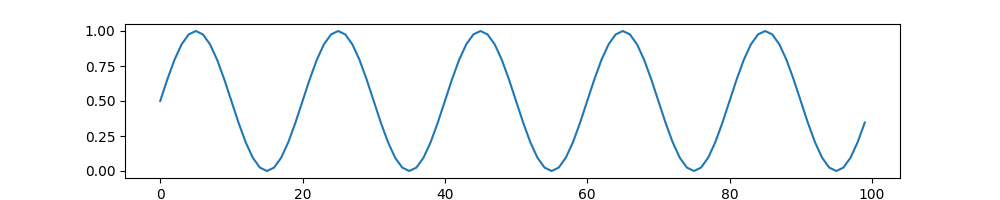
\includegraphics[width=0.95\textwidth, trim={2cm 0cm 2cm 0cm}]{img/projections/signal.png}} \\
%        \fbox{
\includegraphics[width=\projectionsWidth]{img/projections/GramianAngularFieldDifference.png}}
%         & \fbox{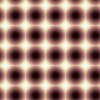
\includegraphics[width=\projectionsWidth]{img/projections/GramianAngularFieldSummation.png}}
%         & \fbox{
\includegraphics[width=\projectionsWidth]{img/projections/MarkovTransitionField.png}}
%         & \fbox{
\includegraphics[width=\projectionsWidth]{img/projections/RecurrencePlot.png}}\\
%        \fbox{
\includegraphics[width=\projectionsWidth]{img/projections/PoincatePlotLogarithmGrid.png}}
%        & \fbox{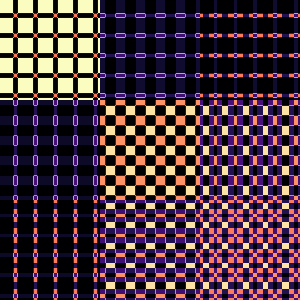
\includegraphics[width=\projectionsWidth]{img/projections/MultiscaleMarkovTransitionField.png}}
%        & \fbox{
\includegraphics[width=\projectionsWidth, height=\projectionsWidth]{img/projections/ShortTimeFFT.png}}
%        & ~ \\
%    \end{tabular}
%    }
%    \egroup
%   	\caption[A signal and its various projection obtained by several methods.]{A signal and its various projection obtained by several methods. In the first line, from the left to the right, the methods are: Gramian Angular Diference Field~\cite{gaf-mtf-1}, Gramian Angular Summation Field~\cite{gaf-mtf-1}, Markov Transition Field~\cite{gaf-mtf-1} and Recurrence Plot~\cite{rp-1}. The methods of the second line are, from the left to the right: Poincaré Plot Density Map~\cite{ecg-6}, Multiscale Markov Transition Field~\cite{imaging-6} and Short Time Fourier Transform Spectogram~\cite{STFT, imaging-1}.}
	\subfigure[]{
		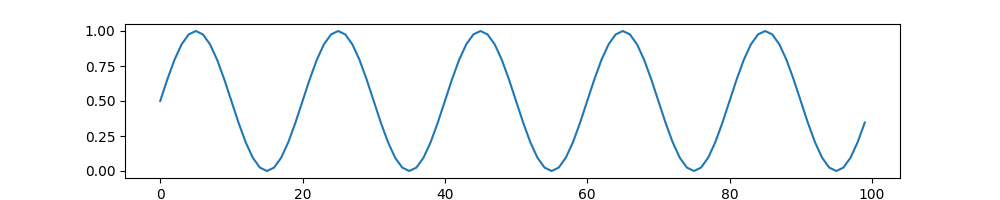
\includegraphics[width=0.95\textwidth]{img/projections/signal.png}
		\label{fig:projections:signal}
	}\\
	\subfigure[]{
		
\includegraphics[width=\projectionsWidth]{img/projections/GramianAngularFieldDifference.png}
		\label{fig:projections:GramianAngularFieldDifference}
	}
	\subfigure[]{
		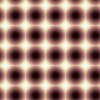
\includegraphics[width=\projectionsWidth]{img/projections/GramianAngularFieldSummation.png}
		\label{fig:projections:GramianAngularFieldSummation}
	}
	\subfigure[]{
		
\includegraphics[width=\projectionsWidth]{img/projections/MarkovTransitionField.png}
		\label{fig:projections:MarkovTransitionField}
	}
	\subfigure[]{
		
\includegraphics[width=\projectionsWidth]{img/projections/RecurrencePlot.png}
		\label{fig:projections:RecurrencePlot}
	}\\
	\subfigure[]{
		
\includegraphics[width=\projectionsWidth]{img/projections/PoincatePlotLogarithmGrid.png}
		\label{fig:projections:PoincatePlotLogarithmGrid}
	}
	\subfigure[]{
		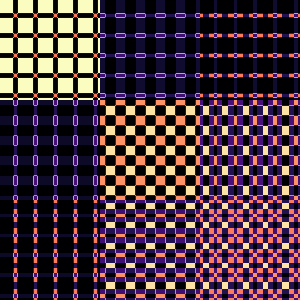
\includegraphics[width=\projectionsWidth]{img/projections/MultiscaleMarkovTransitionField.png}
		\label{fig:projections:MultiscaleMarkovTransitionField}
	}
	\subfigure[]{
		
\includegraphics[width=\projectionsWidth]{img/projections/ShortTimeFFT.png}
		\label{fig:projections:ShortTimeFFT}
	}\\
   	\caption[A signal and its various projection obtained by several methods.]{
   		A signal~\subref{fig:projections:signal} and its various projection obtained by several methods. They are: 
   		\subref{fig:projections:GramianAngularFieldDifference}~Gramian Angular Diference Field~\cite{gaf-mtf-1}, 
   		\subref{fig:projections:GramianAngularFieldSummation}~Gramian Angular Summation Field~\cite{gaf-mtf-1}, 
   		\subref{fig:projections:MarkovTransitionField}~Markov Transition Field~\cite{gaf-mtf-1} and 
   		\subref{fig:projections:RecurrencePlot}~Recurrence Plot~\cite{rp-1}, 
   		\subref{fig:projections:PoincatePlotLogarithmGrid}~Poincaré Plot Density Map~\cite{ecg-6}, 
   		\subref{fig:projections:MultiscaleMarkovTransitionField}~Multiscale Markov Transition Field~\cite{imaging-6} and 
   		\subref{fig:projections:ShortTimeFFT}~Short Time Fourier Transform Spectogram~\cite{STFT, imaging-1}.
   	}
    	\label{fig:literature_projections}
\end{figure}


One particular method present in the \gls{SQA} literature is the time series matrix embedding, which encodes time relationships of the original signal into a square matrix. For instance, Freitas et al. \cite{imaging-4} fed a Vision Transformer with a \gls{RP} or a \gls{MTF}, achieving, respectively, 89.9\% and 90.3\% accuracy on a private dataset. Freitas et al. \cite{imaging-5} also fed images with a Vision Transformer, but used \glspl{GAF}. The proposed approach reached 92.2\% accuracy on a private dataset. Liu et al. \cite{imaging-6} proposed \change{to input} Multiscale Markov Transition Fields, \gls{MTF} version which concatenates the signal first and second derivatives, \change{to} a self-made \gls{CV} model. Experiments with pre-training on the MIMIC-III and UCI databases, and fine-tuning and testing on the Queensland dataset resulted in 99.1\% accuracy for binary classification. Thus, the combination of a generic \gls{CV} model with a projection method, such as \gls{RP}, \gls{GAF} or \gls{MTF}, can achieve a decent accuracy, while it is possible to apply the multiscaling technique to improve some of those projections accuracy. 


\section{Final considerations}
\label{sec:considerations}

Accurate identification of \gls{PPG} sequences contaminated with artifacts is crucial for enabling reliable smart health applications, and \gls{ML} techniques have brought outstanding progress in the field. Nevertheless, \change{none of the previous studies presented in this chapter have} provided an in-depth discussion of these methods. This chapter synthesized the current state-of-the-art approaches applying \gls{ML} algorithms to assess \gls{PPG} signals. Even though there are only a few datasets where signal data are labeled, supervised learning models are more used than their unsupervised counterparts, with \gls{SVM} and \gls{CNN} being the most
widely. Although feature-engineered and deep learning methods demonstrate similar performance levels in some scenarios, deep learning may be more advantageous for addressing the limitations of manual feature engineering. \change{In the current literature, there is also a need for a standardized series of experiments to test and validate the 2D \gls{DL} approach against 1D \gls{ML} methods.} This thesis describes our efforts to fill that gap by experimenting with various existing methods for time series, aiming to conduct a comprehensive study of the field.
